\documentclass[a4wide,11pt]{article}
\usepackage{graphicx}
\usepackage{hyperref}
%\usepackage{a4wide}
\usepackage[a4paper, top=2cm, bottom=2cm, left=2cm, right=2cm]{geometry}
\usepackage{amsbsy,amsmath,amsfonts,amssymb,amsthm,amstext,amscd,amsxtra,amsopn}
\usepackage[]{subfigure}

%%%%%%%%%%%%%%%%%%%%%%%%%%%%%%%%%%%%%%%%%%%%%%%%%%%%%%%%%%%%%%%%%%%%%%%%%%%%%%%%%%%%%%%%%%%%%
\renewcommand{\Re}[1]{\mathrm{Re}{\{#1\}}}
\renewcommand{\Im}[1]{\mathrm{Im}{\{#1\}}}
\renewcommand{\vec}[1]{\mathbf{#1}}
\newcommand{\bc}[1]{\boldsymbol{\mathcal{#1}}}
\newcommand{\hankel}[2]{\mathrm{H}_{#1}^{(#2)}}
\newcommand{\bessel}[1]{\mathrm{J}_{#1}}
\newcommand{\hankelk}[1]{\mathrm{K}_{#1}}
\newcommand{\neumann}[1]{\mathrm{N}_{#1}}
\newcommand{\sgn}[1]{\mathrm{sgn}{(#1)}}
\newcommand{\trint}[2]{\mathop{{\iiint}}\limits_{\!\!\!\!\!\!#1}^{\quad\!#2}}
\newcommand{\dbint}[2]{\mathop{{\iint}}\limits_{\!\!\!\!\!\!#1}^{\quad\!#2}}
\newcommand{\dyad}[1]{\underline{\underline{\mathbf{#1}}}}
\newcommand{\univec}[1]{\mathbf{\hat{#1}}}
\newcommand{\mat}[1]{[\mathbf{#1}]}
\newcommand{\matvec}[1]{\{\mathbf{#1}\}}
\newcommand{\matrow}[1]{(\mathbf{#1})}
%%%%%%%%%%%%%%%%%%%%%%%%%%%%%%%%%%%%%%%%%%%%%%%%%%%%%%%%%%%%%%%%%%%%%%%%%%%%%%%%%%%%%%%%%%%%%
\date{}
\begin{document}

\title{DEMCEM: a Matlab/C++ package for the computation of singular integrals arising in Galerkin EM SIE formulations }
\author{%
Athanasios G. Polimeridis}

\maketitle

\thispagestyle{empty}

\begin{abstract}
Direct Evaluation Method in Computational ElectroMagnetics \href{http://lema.epfl.ch/Members/thanos/Software.html}{DEMCEM} is a package in both Matlab and C++ for the accurate and efficient evaluation of singular integrals arising in Galerkin EM surface integral equation formulations over triangular tessellations. All aspects of the algorithms implemented in this package have been described in the articles found in references [1-4].
\end{abstract}

\section{Introduction}

The main building blocks in EM SIE formulations are the (electric) \textit{Maxwell single layer potential}
\begin{equation}
\bc{L}(\vec{f})(\vec{r}) := ik\bc{S}(\vec{f})(\vec{r}) - \frac{1}{ik} \nabla \mathcal{S}(\nabla'_s \cdot \vec{f})(\vec{r})
\end{equation}
and the (electric) \textit{Maxwell double layer potential}
\begin{equation}
\bc{K}(\vec{f})(\vec{r}) := \nabla\times\bc{S}(\vec{f})(\vec{r})
\end{equation}
where
\begin{equation}
\bc{S}(\vec{f})(\vec{r}) := \int\limits_\Gamma G(\vec{r},\vec{r'}) \vec{f}(\vec{r'}) dS'
\end{equation}
and
\begin{equation}
\mathcal{S}(f)(\vec{r}) := \int\limits_\Gamma G(\vec{r},\vec{r'}) f(\vec{r'}) dS'
\end{equation}
are the associated single layer (acoustic) potentials. Also, $\vec{r}\notin \Gamma$ and $G(\vec{r},\vec{r'})= e^{-ik|\vec{r}-\vec{r'}|} / 4\pi|\vec{r}-\vec{r'}|$ is the homogeneous Green's function.

Following a Galerkin discretization method over planar triangular tessellations, we encounter the evaluation of the following singular integrals:
\begin{equation}\label{I_WS}
\begin{split}
(I_{\bc{L}}^l)_{m,n}:=  ik\int_{E_P} \vec{f}_m\cdot\int_{E_Q}G\;\vec{f}_n\;dS' dS
 + \frac{1}{ik} \int_{E_P} \nabla_s\cdot\vec{f}_m \int_{E_Q} G\, \nabla_s^{'}\cdot\vec{f}_n\;dS' dS
\end{split}
\end{equation}
and
\begin{equation}\label{I_SS}
(I_{\bc{K}}^p)_{m,n}:= \int_{E_P} \vec{f}_m \cdot\int_{E_Q}\nabla G\, \times \vec{f}_n\;dS' dS
\end{equation}
where $l\in \{{\rm ST,EA,VA}\}$ and $p\in \{{\rm EA,VA}\}$ stand for the cases of coincident (or self-term, ST), edge adjacent (EA) and vertex adjacent (VA) observation and source triangles, $E_P$ and $E_Q$, respectively.

\section{Weakly Singular Integrals}


DIRECT\textunderscore WS\textunderscore\{ST,EA,VA\}\textunderscore RWG subfolders contain codes for the evaluation of the weakly singular integrals $(I_{\bc{L}}^l)_{m,n}$. The basic output parameters for all three cases are given as follows:
\begin{equation*}
\begin{split}
I_{\rm DE}(1) \rightarrow (I_{\bc{L}}^l)_{1,1} \\
I_{\rm DE}(2) \rightarrow (I_{\bc{L}}^l)_{1,2}\\
I_{\rm DE}(3) \rightarrow (I_{\bc{L}}^l)_{1,3} \\
I_{\rm DE}(4) \rightarrow (I_{\bc{L}}^l)_{2,1} \\
I_{\rm DE}(5) \rightarrow (I_{\bc{L}}^l)_{2,2} \\
I_{\rm DE}(6) \rightarrow (I_{\bc{L}}^l)_{2,3} \\
I_{\rm DE}(7) \rightarrow (I_{\bc{L}}^l)_{3,1} \\
I_{\rm DE}(8) \rightarrow (I_{\bc{L}}^l)_{3,2} \\
I_{\rm DE}(9) \rightarrow (I_{\bc{L}}^l)_{3,3}
\end{split}
\end{equation*}
omitting the constant $1/4\pi$ in homogeneous Green's function $G$! Basis and testing functions are the traditional RWG. \texttt{EXAMPLE$\_$WS$\_$\{ST,EA,VA\}$\_$RWG.m} scripts are used as examples to call the main codes:
\begin{itemize}
\item Self-term

\texttt{I$\_$DE = DIRECT$\_$WS$\_$ST$\_$RWG(r1,r2,r3,Np$\_$1D)}
\item Edge adjacent

\texttt{I$\_$DE = DIRECT$\_$WS$\_$EA$\_$RWG(r1,r2,r3,r4,Np$\_$theta,Np$\_$psi)}
\item Vertex adjacent

\texttt{I$\_$DE = DIRECT$\_$WS$\_$VA$\_$RWG(r1,r2,r3,r4,r5,Np$\_$theta$\_$p,Np$\_$theta$\_$q,Np$\_$psi)}
\end{itemize}
Note that the nodes of the associated triangles, especially for the EA and VA cases, follow the orientation depicted in Fig.1 (a) and (b), respectively. Wavenumber, denoted as \texttt{$k_o$} is declared as a global variable. Moreover, it is better to keep the same order for 1-D quadratures in EA and VA cases, i.e., \texttt{Np$\_$theta$=$Np$\_$psi} and \texttt{Np$\_$theta$\_$p$=$Np$\_$theta$\_$q$=$Np$\_$psi}. Detailed comments regarding the input and output parameters are also provided in each separate main function.

%%%%%%%%%%%%%%%%%%%%%%%%%%%%%%%%%%%%%%%%%%%%%%%%%%%%%%%%%%%%%%%%%%%%%%%%%%%%%
%                             FIGURE
%%%%%%%%%%%%%%%%%%%%%%%%%%%%%%%%%%%%%%%%%%%%%%%%%%%%%%%%%%%%%%%%%%%%%%%%%%%%%
\begin{figure}
\begin{center}
\subfigure[Edge-adjacent case.]{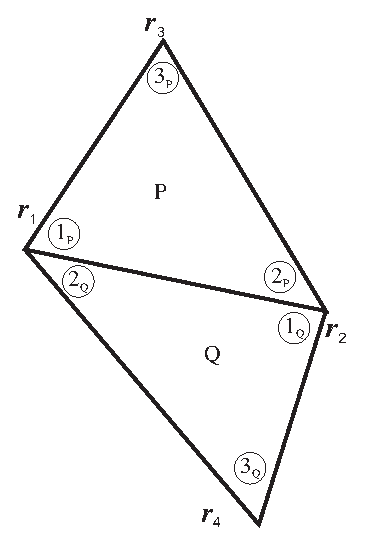
\includegraphics[scale=0.8]{figure1.eps}\label{fig.a}}
\hfil \subfigure[Vertex-adjacent case.]{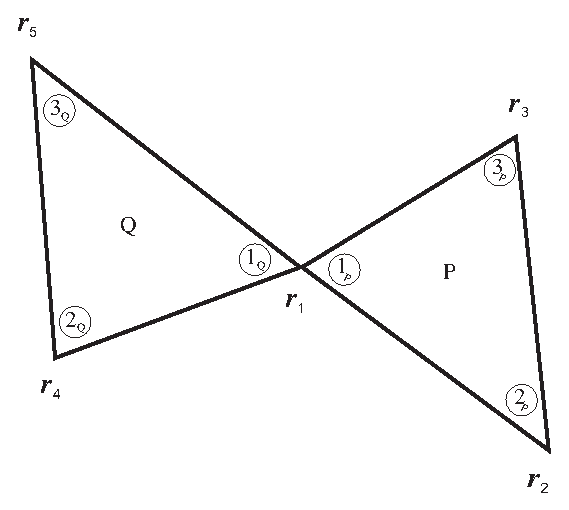
\includegraphics[scale=0.8]{figure2.eps}\label{fig.b}}
\end{center}
\caption{Orientation of the triangular elements in DEMCEM.}\label{fig}
\end{figure}
%%%%%%%%%%%%%%%%%%%%%%%%%%%%%%%%%%%%%%%%%%%%%%%%%%%%%%%%%%%%%%%%%%%%%%%%%%%%%

\section{Strongly Singular Integrals}

\texttt{DIRECT$\_$SS$\_$\{EA,VA\}$\_$\{RWG,nxRWG\}} subfolders contain codes for the evaluation of the strongly singular integrals $(I_{\bc{K}}^p)_{m,n}$ with RWG and nxRWG testing functions. In all cases, RWG basis functions are considered. Also, EA and VA stand for the edge adjacent and vertex adjacent triangles (coincident integrals' case is identically zero).

The basic output parameters for both cases are given as follows:
\begin{equation*}
\begin{split}
I_{\rm DE}(1) \rightarrow (I_{\bc{K}}^p)_{1,1} \\
I_{\rm DE}(2) \rightarrow (I_{\bc{K}}^p)_{1,2}\\
I_{\rm DE}(3) \rightarrow (I_{\bc{K}}^p)_{1,3} \\
I_{\rm DE}(4) \rightarrow (I_{\bc{K}}^p)_{2,1} \\
I_{\rm DE}(5) \rightarrow (I_{\bc{K}}^p)_{2,2} \\
I_{\rm DE}(6) \rightarrow (I_{\bc{K}}^p)_{2,3} \\
I_{\rm DE}(7) \rightarrow (I_{\bc{K}}^p)_{3,1} \\
I_{\rm DE}(8) \rightarrow (I_{\bc{K}}^p)_{3,2} \\
I_{\rm DE}(9) \rightarrow (I_{\bc{K}}^p)_{3,3}
\end{split}
\end{equation*}

Note again that the constant $1/4\pi$ in homogeneous Green's function $G$ is omitted!

\texttt{EXAMPLE$\_$SS$\_$\{ST,EA,VA\}$\_$\{RWG,nxRWG\}.m} scripts are used as examples to call the main codes:

\begin{itemize}

\item Edge adjacent with RWG tesing functions

\texttt{I$\_$DE = DIRECT$\_$SS$\_$EA$\_$RWG(r1,r2,r3,r4,Np$\_$theta,Np$\_$psi)}

\item Edge adjacent with nxRWG tesing functions

\texttt{I$\_$DE = DIRECT$\_$SS$\_$EA$\_$nxRWG(r1,r2,r3,r4,Np$\_$theta,Np$\_$psi)}

\item Vertex adjacent with RWG tesing functions

\texttt{I$\_$DE = DIRECT$\_$SS$\_$VA$\_$RWG(r1,r2,r3,r4,r5,Np$\_$theta$\_$p,Np$\_$theta$\_$q,Np$\_$psi)}

\item Vertex adjacent with nxRWG tesing functions

\texttt{I$\_$DE = DIRECT$\_$SS$\_$VA$\_$nxRWG(r1,r2,r3,r4,r5,Np$\_$theta$\_$p,Np$\_$theta$\_$q,Np$\_$psi)}

\end{itemize}

Detailed comments regarding the input and output parameters are also provided in the Section 2 as well as in each separate main function.

\section{Implementation in C}

DEMCEM package in C follows the same philosophy as the Matlab version presented above, but typically runs $\approx$15-30 faster, depending on the case.


\section{Matlab plugins}

This package also includes source code for compiled Matlab plugins
(MEX files) to provide a fast Matlab interface to this functionality.
Given a C compiler, simply run the provided script


      \texttt{mexDEMCEM$\_$build}


\noindent in Matlab. This will compile all functions with \texttt{mex} prefix. Note that the input arguments are different in this case (include weights and points of the 1-D GL quadratures)!


\section*{Licence}

Copyright \copyright 2013 Athanasios Polimeridis
\\\\
\noindent DEMCEM is free software; you can redistribute it and/or modify it under the terms of the GNU Lesser General Public License (LGPL) as published by the Free Software Foundation; either version 3 of the License, or (at your option) any later version.
\\\\
\noindent DEMCEM is distributed in the hope that it will be useful, but WITHOUT ANY WARRANTY; without even the implied warranty of MERCHANTABILITY or FITNESS FOR A PARTICULAR PURPOSE. See the GNU GPLv3 for more details.
\\\\
\noindent You should have received a copy of the GNU General Public License along with this program. If not, see http://www.gnu.org/licenses/.

\begin{thebibliography}{9}
\itemsep=0ex

\bibitem{Polimeridis2008} A. G. Polimeridis and T. V. Yioultsis, ``On the direct evaluation of weakly singular integrals in Galerkin mixed potential integral equation formulations'', \textit{IEEE Trans. Antennas Propag.}, vol. 56, no. 9, pp. 3011-3019, Sep. 2008.

\bibitem{Polimeridis2010} A. G. Polimeridis and J. R. Mosig, ``Complete semi-analytical treatment of weakly singular integrals on planar triangles via the direct evaluation method'', \textit{Int. J. Numerical Methods Eng.}, vol. 83, pp. 1625-1650, 2010.

\bibitem{Polimeridis2011} A. G. Polimeridis, J. M. Tamayo, J. M. Rius, and J. R. Mosig, ``Fast and accurate computation of hyper-singular integrals in Galerkin surface integral equation formulations via the direct evaluation method'', \textit{IEEE Trans. Antennas Propag.}, vol. 59, no. 6, pp. 2329-2340, Jun. 2011.

\bibitem{Polimeridis2011b} A. G. Polimeridis and J. R. Mosig, ``On the direct evaluation of surface integral equation impedance matrix elements involving point singularities'', \textit{IEEE Antennas Wireless Propag. Lett.}, vol. 10, pp. 599-602, 2011.

\end{thebibliography}


\end{document}
